%{The position of a point after a rotation about the origin can be calculated simply by multiplying its coordinates by a matrix. One reason for using homogeneous coordinates is to be able to describe translation with a matrix, so that multiple transformations, whether rotations or translations, can be concatenated into one described by the product of their respective matrices. However, in some applications (such as satellite tracking), we only need to be concerned with an object's rotations, or at least separately from other transformations. In such cases, we frequently need to extract the rotation axis and angle from a matrix that represents the concatenation of multiple rotations. The homogeneous transformation matrix, on the other hand, is inadequate for the task.}%

\section{Direction Cosine Matrix}

Three-dimensional space, denoted $\mathbb{R}^3$, can be coordinated in a manner that is entirely analogous to how coordinates in $\mathbb{R}^2$ are introduced. $\mathbb{R}^3$ specifies an arbitrary but fixed point, which we call the origin. Three mutually perpendicular lines passing through this origin are designated as the \textit{x-axis,y-axis,and z-axis} respectively. Each of these axes is a real number line, with the origin at the zero point. These axes are oriented so that a positive or right-handed coordinate frame is formed. A right-handed coordinate frame is one in which the right hand's fingers point positively along the \textit{x-axis.}


Given such a 3D coordinate system, points are represented by triplets of real numbers $(x, y, z)$. The origin point $O$ is represented in this frame by the point $(0, 0, 0)$. Any given point in this coordinate system can be represented as $P(x,y,z)$ which also can be represented as vector v from the origin $O$ to the point $P$.


In $\mathbb{R}^3$, a rotation vector or axis that remains fixed during the rotation (such as x, y and z axes) is needed to rotate about. In this case, the rotation matrix $[\textbf{A}]$ can be described as a 3×3 matrix. Suppose that a vector has coordinates $(x_1, y_1, z_1)$ relative to the \textit{xyz} coordinate frame. If the coordinate frame is rotated with an angle $\theta$ about the \textit{x-axis}. Let the coordinates $(x_2, y_2, z_2)$ denotes $P$ in the rotated frame. As the rotation occurs about \textit{z-axis}, the z component will not be affected by the rotation. 
$$z_1=z_2$$

$x_2$ and $y_2$ are determined by the following equations
\begin{equation}
\begin{gathered}
x_{2}=\cos (\theta) x_{1}+\sin (\theta) y_{1}+0 z_{1} \\
y_{2}=-\sin (\theta) x_{1}+y_{1} \cos (\theta)+0 z_{1} \\
z_{2}=0 x_{1}+0 y_{1}+z_{1}
\end{gathered}
\end{equation}
This can be represented as 
\begin{equation}
\left[\begin{array}{l}
x_{2} \\
y_{2} \\
z_{2}
\end{array}\right]=\left[\begin{array}{ccc}
\cos (\theta) & \sin (\theta) & 0 \\
-\sin (\theta) & \cos (\theta) & 0 \\
0 & 0 & 1
\end{array}\right]\left[\begin{array}{l}
x_{1} \\
y_{1} \\
z_{1}
\end{array}\right]
\end{equation}
Now, the rotation in $\mathbb{R}^3$  by angle $\theta$ about the \textit{z-axis} can be carried out using the rotation matrix represented
\begin{equation}
R(\theta)=\left[\begin{array}{ccc}
\cos (\theta) & \sin (\theta) & 0 \\
-\sin (\theta) & \cos (\theta) & 0 \\
0 & 0 & 1
\end{array}\right]
\end{equation}
This matrix is also called the direction cosine matrix.
\section{Euler angles}
A rigid body in space has a coordinate frame attached to it, which is frequently located at the center of mass. This frame is known as the body frame or the local frame. The body frame can be used to describe the position, orientation, and motion of the body in relation to a fixed reference frame known as the Inertial frame as in figure \ref{fig:reff}.
\tdplotsetmaincoords{70}{140}

\begin{figure}[H]
\centering
\begin{tikzpicture}[tdplot_main_coords]
\draw[thick,->] (-1,0,0) -- (4,0,0) node[below left] {$ x $};
\draw[thick,->] (0,-1,0) -- (0,4,0) node[below left] {$ y $};
\draw[thick,->] (0,0,-1) -- (0,0,4) node[below left] {$ z $} node[midway, below=2.9cm] {Inertial frame};

\draw[thick, ->,rotate=30] (8,5,8) -- (9,5,8) node[below left] {$ x_b $};
\draw[thick, ->,rotate=30] (8,5,8) -- (8,6,8) node[below left] {$ y_b $};
\draw[thick, ->,rotate=30] (8,5,8) -- (8,5,9) node[below left] {$ z_b $} node[midway, below=1.2cm] {body frame};

\end{tikzpicture}
\caption{Body frame with respect to inertial reference frame.} \label{fig:reff}
\end{figure}


There are six degrees of freedom for the rigid body: its position in the world frame is given by the \textit{x,y,and z} coordinates of its center of mass such as the origin of the local frame, and its orientation defined by three angles of rotation of its body frame relative to the world frame One option for describing this rotation is to use three angles, one for each of the world frame's \textit{x-,y-,and z-axes}. From the perspective of the rotating body, using three angles about the body frame's axes is a more convenient option. The last three angles are known as Euler angles. 
Depending on the axes around which the rotations are performed, there are several conventions for Euler angles. The \textit{XYZ} Euler angles are introduced here. The body frame is initially oriented in the same way as the world frame.
\begin{figure}[H]
    \centering
    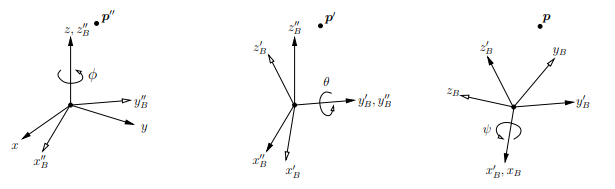
\includegraphics[width = 0.7\textwidth]{Figures/ea2.png}
    \caption{Rotation sequence.}
    \label{fig:ea}
\end{figure}
Three consecutive different rotations are carried out to move from the world frame to the final position. The first rotation is about the body \textit{x–axis} by an angle $\psi$, the second rotation is about the body \textit{y-axis} by an angle $\theta$ and the third rotation is about the body \textit{z–axis} by an angle $\phi$. $\phi$, $\theta$ and $\psi$ are the Euler angles in this case.

\begin{equation}
\begin{gathered}
\boldsymbol{p}^{\prime}=R_{x}(\psi) \boldsymbol{p} \\
\boldsymbol{p}^{\prime \prime}=R_{y}(\theta) R_{x}(\psi) \boldsymbol{p} \\
R_{z}(\phi) \boldsymbol{p}^{\prime \prime}=R_{z}(\phi) R_{y}(\theta) R_{x}(\psi) \boldsymbol{p} \\
R_{x y z}(\psi, \theta, \phi)=R_{z}(\phi) R_{y}(\theta) R_{x}(\psi) \\
\end{gathered}
\end{equation}
The total rotation matrix is defined as
\begin{equation*}
\begin{gathered}
R_{x y z}(\psi, \theta, \phi)=\left[\begin{array}{cccc}
\cos (\phi) & -\sin (\phi) & 0 \\
\sin (\phi) & \cos (\phi) & 0 \\
0 & 0 & 1
\end{array}\right]\left[\begin{array}{ccc}
\cos (\theta) & 0 & \sin (\theta) \\
0 & 1 & 0 \\
-\sin (\theta) & 0 & \cos (\theta)
\end{array}\right]\left[\begin{array}{ccc}
1 & 0 & 0 \\
0 & \cos (\psi) & -\sin (\psi) \\
0 & \sin (\psi) & \cos (\psi)
\end{array}\right]
\end{gathered}
\end{equation*}
\begin{equation}
R_{x y z}(\psi, \theta, \phi)=\left[\begin{array}{ccc}
c \phi c \theta & c \phi s \theta s \psi-s \phi c \psi & c \phi s \theta c \psi+s \phi s \psi \\
s \phi c \theta & s \phi s \theta s \psi+c \phi c \psi & s \phi s \theta c \psi-c \phi s \psi \\
-s \theta & c \theta s \psi & c \theta c \psi
\end{array}\right]
\end{equation}
This is defined as the rotation matrix DCM.

\section{Quaternions}
W. R. Hamilton \cite{hamilton1848xi} is credited with the invention of quaternions in 1843. According to legend, Hamilton was strolling with his wife Helen at the Royal Irish Academy when the thought of adding a fourth dimension to multiply triples hit him. He etched the newfound quaternion equations 
\begin{equation}
    \hat{\boldsymbol{i}}^{2}=\hat{\boldsymbol{\jmath}}^{2}=\hat{\boldsymbol{k}}^{2}=\hat{\boldsymbol{\imath}}\hat{\boldsymbol{j}} \hat{\boldsymbol{k}}=-1
\end{equation}
into the stone as he and his wife passed the Brougham bridge of the Royal Canal.
His problem was to find a similar analogy to what is known for the complex number in $\mathbb{R}^2$. The Product of complex numbers in $\mathbb{R}^2$ geometrically provoked into the rotation of vectors in the plane. Hamilton needed to find such a way in $\mathbb{R}^3$ space using real number triplets. His way discussed in earlier equation managed to have such an implication \cite{kuipers1999quaternions}. 

\subsection{Definition}
Let an expression of the form
\begin{equation}\label{q_quat}
    q=q_{0}+q_{1} \hat{\imath}+q_{2} \hat{\jmath}+q_{3} \hat{k} \quad \Leftrightarrow \quad q=q_{0}+\boldsymbol{q}
\end{equation}
Be called a quaternion where  $q_1,q_2,q_3,q_4$ are the four constituents of the quaternion $q$, denote any real quantities, positive or negative or null, but $\hat{i}, \hat{j}, \hat{k}$ are symbols of three imaginary quantities, which we shall call imaginary units, and are assumed to be unconnected by any linear relation with each other.

From the definition we see that we can set in complex numbers $\mathbb{Z}$, and thus real $\mathbb{R}$ and imaginary numbers $\mathbb{I}$, in the quaternion Hamilton space $\mathbb{H}$, in the sense that real, imaginary and complex numbers are implicitly quaternions
\begin{equation}
q=q_{0} \in \mathbb{R} \subset \mathbb{H}, \quad q=q_{1} \hat{\imath} \in \mathbb{I} \subset \mathbb{H}, \quad q=q_{0}+q_{1} \hat{\imath} \in \mathbb{Z} \subset \mathbb{H}
\end{equation}

Similarly, we can define numbers in $\mathbb{H}$'s three-dimensional imaginary subspace. They can be called pure quaternions, and the space of pure quaternions is $\mathbb{H}_p=Im(\mathbb{H})$ 
\begin{equation}
    q=q_{1} \hat{\imath}+q_{2} \hat{\jmath}+q_{3} \hat{k} \in \mathbb{H}_p \subset \mathbb{H} 
\end{equation}
A quaternion can be defined as an order pair scalar-vector
\begin{equation}
\left\langle q_{0}, \boldsymbol{q}\right\rangle
\end{equation}
Quaternions are defined frequently as a 4-vector q as
\begin{equation}
\boldsymbol{q} \triangleq\left[\begin{array}{c}
q_{0} \\
\boldsymbol{q}
\end{array}\right]=\left[\begin{array}{l}
q_{0} \\
q_{1} \\
q_{2} \\
q_{3}
\end{array}\right]
\end{equation}
This allows us to utilize matrix algebra for quaternion operations. We might allow ourselves to blend notations on occasion by manipulating the symbol (=).
\subsection{Quaternions Equality, Addition, and Subtraction}
If there is another quaternion
\begin{equation}
    q'=q'_{0}+q'_{1} \hat{\imath}+q'_{2} \hat{\jmath}+q'_{3} \hat{k} \quad \Leftrightarrow \quad q'=q'_{0}+\boldsymbol{q'}
\end{equation}
the presumption that these two quaternions are equal,
\begin{equation}
    q'=q
\end{equation}
shall be considered to entail four independent equations between their elements, namely, the four equations listed below
\begin{equation}
\begin{gathered}
q_{1}^{\prime}=q_{1}, \quad q_{2}^{\prime}=q_{2}, \quad q_{3}^{\prime}=q_{3}, \quad q_{4}^{\prime}=q_{4}
\end{gathered}
\end{equation}
It will then be natural to state that the formula affects the addition and subtraction of quaternions as
\begin{equation}
\begin{gathered}
q \pm q^{\prime}=\left(q_{0}^{\prime} \pm q_{0}\right)+\left(q_{1}^{\prime} \pm q_{1}\right) \hat{\imath}+\left(q_{2}^{\prime} \pm q_{2}\right) \hat{\jmath}+\left(q_{3}^{\prime} \pm q_{3}\right) \hat{k} \Leftrightarrow q \pm q^{\prime}=\left(q_{0}^{\prime} \pm q_{0}\right)+\left(\boldsymbol{q}+\boldsymbol{q}^{\prime}\right)
\end{gathered}
\end{equation}
or, to say with different way, by the rule that the sums or differences of the constituents of any two quaternions are the components of the sum or difference of those two quaternions.
\subsection{Quaternions Multiplication}
As in $\mathbb{R}^3$ , the product of a scalar and a quaternion is defined in the same way as vectors are defined. If $c$ is a scalar and $q$ is a quaternion. The result is the product of the quaternion $q$ and the scalar $c$ is
\begin{equation}
cq=cq_{0}+cq_{1} \hat{\imath}+cq_{2} \hat{\jmath}+cq_{3} \hat{k} \quad \Leftrightarrow \quad q=cq_{0}+c\boldsymbol{q}
\end{equation}
Simply multiply the quaternion's components by the scalar to multiply the quaternion by the scalar. It's worth noticing that the result is another quaternion.

Given the fundamental set of rules proposed by Hamilton 
\begin{equation}
\begin{gathered}
\hat{\boldsymbol{i}}^{2}=\hat{\boldsymbol{\jmath}}^{2}=\hat{\boldsymbol{k}}^{2}=\hat{\boldsymbol{\imath}}\hat{\boldsymbol{j}} \hat{\boldsymbol{k}}=-1 \\
\hat{\boldsymbol{\jmath}} \hat{\boldsymbol{j}}=\hat{\boldsymbol{k}}=-\hat{\boldsymbol{\jmath}} \hat{\boldsymbol{i}} \\
\hat{\boldsymbol{\jmath}} \hat{\boldsymbol{k}}=\hat{\boldsymbol{i}}=-\hat{\boldsymbol{k}} \hat{\boldsymbol{J}} \\
\hat{\boldsymbol{k}} \hat{\boldsymbol{\imath}}=\hat{\boldsymbol{j}}=-\hat{\boldsymbol{\imath}} \hat{\boldsymbol{k}}
\end{gathered}
\end{equation}
It will also be natural to state that the product $qq^{'}$, which is the result of multiplying $q_1$ as a multiplier into $q^'$  as a multiplicand, can be formulated as
\begin{equation}
\begin{aligned}
&q q^{\prime}=\left(q_{0}+q_{1} \hat{\imath}+q_{2} \hat{\jmath}+q_{3} \hat{k}\right)\left(q_{0}^{\prime}+q_{1}^{\prime} \hat{\imath}+q_{2}^{\prime} \hat{\jmath}+q_{3}^{\prime} \hat{k}\right) \\
&=\left(q_{0} q_{0}^{\prime}\right)-\left(q_{1} q_{1}^{\prime}+q_{2} q_{2}^{\prime}+q_{3} q_{3}^{\prime}\right)+q_{0}\left(q_{1}^{\prime} \hat{\imath}+q_{2}^{\prime} \hat{\jmath}+q_{3}^{\prime} \hat{k}\right) \\
&+q_{0}^{\prime}\left(q_{1} \hat{\imath}+q_{2} \hat{\jmath}+q_{3} \hat{k}\right)+\hat{\imath}\left(q_{2} q_{3}^{\prime}-q_{3} q_{2}^{\prime}\right)+\hat{\jmath}\left(q_{3} q_{1}^{\prime}-q_{1} q_{3}^{\prime}\right)+\hat{k}\left(q_{1} q_{2}^{\prime}-q_{2} q_{1}^{\prime}\right) \\
\end{aligned}
\end{equation}
\begin{equation}
\begin{aligned}
q q^{\prime}=\left[\begin{array}{l}
q_{0} q_{0}^{\prime}-q_{1} q_{1}^{\prime}-q_{2} q_{2}^{\prime}-q_{3} q_{3}^{\prime} \\
q_{0} q_{1}^{\prime}+q_{0}^{\prime} q_{1}+q_{2} q_{3}^{\prime}-q_{3} q_{2}^{\prime} \\
q_{0} q_{2}^{\prime}+q_{0}^{\prime} q_{2}+q_{3} q_{1}^{\prime}-q_{1} q_{3}^{\prime} \\
q_{0} q_{3}^{\prime}+q_{0}^{\prime} q_{3}+q_{1} q_{2}^{\prime}-q_{2} q_{1}^{\prime}
\end{array}\right]=\left[\begin{array}{c}
q_{0} q_{0}^{\prime}-\boldsymbol{q}^{\top} \boldsymbol{q}^{\prime} \\
q_{0} \boldsymbol{q}^{\prime}+q_{0}^{\prime} \boldsymbol{q}+\boldsymbol{q} \times \boldsymbol{q}^{\prime}
\end{array}\right]
\end{aligned}
\end{equation}
Utilizing the inner and cross product of two vector in $\mathbb{R}^3$ in order to rewrite the above expression in more concise form
\begin{equation}
q q^{\prime}=q_{0} q_{0}^{\prime}-\boldsymbol{q} \cdot \boldsymbol{q}^{\prime}+q_{0} \boldsymbol{q}+q_{0}^{\prime} \boldsymbol{q}+\boldsymbol{q} \times \boldsymbol{q}^{\prime}
\end{equation}

\subsection{Quaternion Complex Conjugate and the Norm}
The complex conjugate of a quaternion, an important algebraic notion relevant to quaternions as well as conventional complex numbers, will be beneficial in what follows.
Let $q$ be a quaternion defined in (\ref{q_quat}). The conjugate of $q$ will be donated as $\bar{q}$ and is defined as
\begin{equation}\label{q_quat_con}
    \bar{q}=q_{0}-q_{1} \hat{\imath}-q_{2} \hat{\jmath}-q_{3} \hat{k} \quad \Leftrightarrow \quad \bar{q}=q_{0}-\boldsymbol{q}
\end{equation}
From the definition we consequently have the following
\begin{equation*}
\begin{gathered}
\overline{(\bar{q})}=\overline{\left(q_{0}-\boldsymbol{q}\right)}=\left(q_{0}+\boldsymbol{q}\right)=q,\\
    \bar{q}+q=2 q_{0}
\end{gathered}
\end{equation*}
The norm of a quaternion $q$, denoted by 
\begin{equation}
\norm{q}\triangleq\sqrt{q \bar{q}}
\end{equation}
\begin{equation}
\begin{gathered}
\bar{q} q=\left(q_{0}-\boldsymbol{q}\right)\left(q_{0}+\boldsymbol{q}\right) \\
=q_{0} q_{0}-(-\boldsymbol{q}) \cdot \boldsymbol{q}+q_{0} \boldsymbol{q}+(-\boldsymbol{q}) q_{0}+(-\boldsymbol{q}) \times \boldsymbol{q}=q_{0}^{2}+\boldsymbol{q} \cdot \boldsymbol{q} \\
=q_{0}^{2}+\boldsymbol{q} \cdot \boldsymbol{q}=q_{0}^{2}+q_{1}^{2}+q_{2}^{2}+q_{3}^{2}=q \bar{q}
\end{gathered}
\end{equation}
\begin{equation}
    \norm{q}=\sqrt{q_{0}^{2}+q_{1}^{2}+q_{2}^{2}+q_{3}^{2}} \in \mathbb{R}
\end{equation}
A quaternion is named a unit or normalized quaternion if it has a norm equals to 1. If a quaternion has norm 1 each of its components must have absolute value less than or equal to one \cite{kuipers1999quaternions}.

\subsection{Natural power and the exponential of pure quaternions}
The quaternion exponential function is a quaternion-based version of the exponential function. It is defined as the totally convergent power series, much like in the real exponential case \cite{sola2017quaternion}.
\begin{equation}
e^{q}=\sum_{k=0}^{\infty} \frac{1}{k !} q^{k} \in \mathbb{I I}
\end{equation}
More remarkably, the exponential representation of a pure quaternion $\boldsymbol{v} = v_1 \hat{\imath}+v_2 \hat{\jmath}+v_3 \hat{\kmath}$ is a new quaternion defined by
\begin{equation}
    e^{v}=\sum_{k=0}^{\infty} \frac{1}{k !} v^{k} \subset \mathbb{I}
\end{equation}
Let us define $q^n, \,n \in \mathbb{N}$, as the \textit{n-th} power of $q$ using the quaternion product. Then, if $\boldsymbol{v}$ is a pure quaternion and we let $\boldsymbol{v}=\hat{\boldsymbol{{a}}} \theta$, with $\theta = \norm{\boldsymbol{v}} \in \mathbb{R}$ and $\hat{\boldsymbol{a}}$  unitary, we get from the definition of quaternion product the cyclic pattern
\begin{equation}\label{eqn:cyc}
v^{2}=-\theta^{2}, \quad v^{3}=-\widehat{\boldsymbol{a}} \theta^{3}, \quad v^{4}=\theta^{4}, \quad v^{5}=\widehat{\boldsymbol{a}} \theta^{5}
\end{equation}
From the cyclic pattern retrieved in (\ref{eqn:cyc}), and grouping the scalar and vector terms in the series
\begin{equation}
    e^{v}=e^{\hat{\boldsymbol{a}} \theta}=\left(1-\frac{\theta^{2}}{2 !}+\frac{\theta^{4}}{4 !}+\cdots\right)+\left(\hat{\boldsymbol{a}} \theta-\frac{\hat{\boldsymbol{a}} \theta^{3}}{3 !}+\frac{\hat{\boldsymbol{a}} \theta^{5}}{5 !}+\cdots\right)
\end{equation}
and recognize in them, correspondingly, the series expansion of $cos\theta, \,\text{and } sin\theta$
\begin{equation}
e^{v}=e^{\hat{a} \theta}=\cos \frac{\theta}{2}+\hat{\boldsymbol{a}} \sin \frac{\theta}{2}=\left[\begin{array}{c}
\cos \frac{\theta}{2} \\
\hat{\boldsymbol{a}} \sin \frac{\theta}{2}
\end{array}\right]
\end{equation}
which establishes a stunning extension of the Euler formula, $e^{i\theta}= cos\theta + i sin\theta$, defined for $\mathbb{I}$. Notice that since $\norm{e^v}^2  =cos^2 \theta+  sin^2 \theta= $1, the exponential representation of a pure quaternion is a unit quaternion.
Consequently, for any unit quaternion
\begin{equation} \label{eqn:sin_cos}
    q=q_0+\boldsymbol{q}=cos\frac{\theta}{2}+\hat{\boldsymbol{a}} sin\frac{\theta}{2}
\end{equation}


\subsection{Rotation Operator}
For any vector $v \in\mathbb{R}^3 \subset \mathbb{H}$ the action of the operator
\begin{equation}
    \mathcal{L}(\boldsymbol{v})=q\boldsymbol{v}\bar{q}
\end{equation}
on $\boldsymbol{v}$ is equivalent to a rotation of the vector through an angle $\theta$ about $\hat{u}$ as the axis of rotation.

The analysis to prove this theorem will be based on getting the expression of the vector $\boldsymbol{w}$, the image of vector $\boldsymbol{v}$ after rotation about the unit quaternion, shown in the figure \ref{fig:rot}, geometrically, then getting an expression using quaternion will be called the quaternion rotation operator.
\begin{figure}[H]
    \centering
    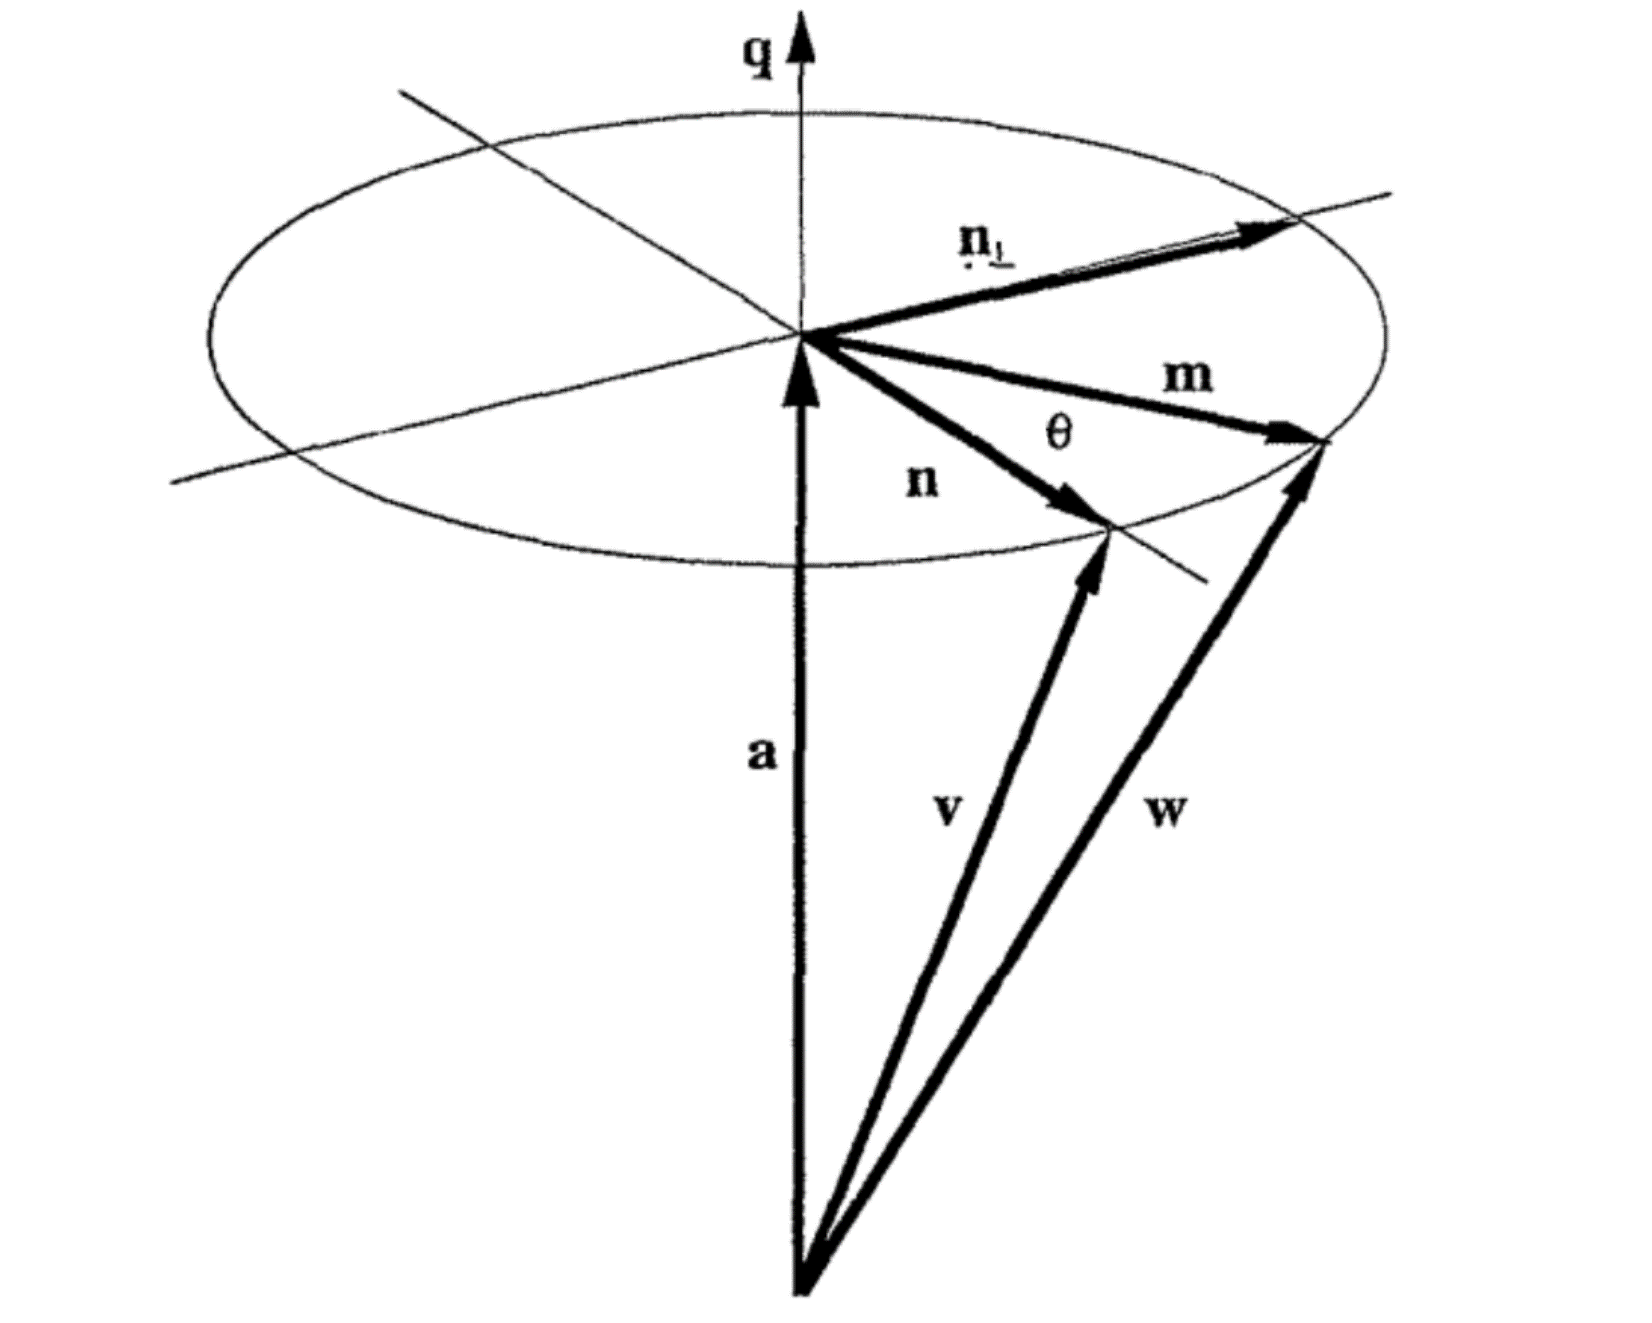
\includegraphics[width=0.5\textwidth]{Figures/rot.png}
    \caption{Vector $\boldsymbol{v}$ rotated with angle $\theta$ to be vector $\boldsymbol{w}$}
    \label{fig:rot}
\end{figure}
\begin{equation}
\boldsymbol{w}=\widehat{\boldsymbol{a}}+\boldsymbol{m} 
\end{equation}
For getting the expression of the vector $\boldsymbol{\hat{a}}$, the projection of $\boldsymbol{v}$ on the direction of $\boldsymbol{\hat{a}}$

\begin{equation*}
    \begin{gathered}
\boldsymbol{a}=(v . \widehat{\boldsymbol{a}}) . \widehat{\boldsymbol{a}} \\
\boldsymbol{n}=\boldsymbol{v}-\widehat{\boldsymbol{a}}=\boldsymbol{v}-(\boldsymbol{v} \cdot \widehat{\boldsymbol{a}}) \cdot \widehat{\boldsymbol{a}} \\
\boldsymbol{n}_{\perp}=\widehat{\boldsymbol{a}} \times \boldsymbol{v} \\
\boldsymbol{m}=\boldsymbol{n} \cos (\theta)+\boldsymbol{n}_{\perp} \sin (\theta)=\cos (\theta)(\boldsymbol{v}-(\boldsymbol{v} \cdot \widehat{\boldsymbol{a}}) \cdot \widehat{\boldsymbol{a}})+\sin (\theta)(\widehat{\boldsymbol{a}} \times \boldsymbol{v})
    \end{gathered}
\end{equation*}
Therefore,
\begin{equation}\label{eqn:geo}
    \boldsymbol{w}=(\boldsymbol{v} . \widehat{\boldsymbol{a}}) \cdot \widehat{\boldsymbol{a}}+\cos (\theta)(\boldsymbol{v}-(\boldsymbol{v} \cdot \boldsymbol{a}) \cdot \widehat{\boldsymbol{a}})+\sin (\theta)(\widehat{\boldsymbol{a}} \times \boldsymbol{v})
\end{equation}
Equation (\ref{eqn:geo}) will be revisited after getting the expression of $\mathcal{L}(\boldsymbol{v})=q\boldsymbol{v}\bar{q}$.
Extending the analysis to calculate the value of the operator $\mathcal{L}(\boldsymbol{v})=q\boldsymbol{v}\bar{q}$.
\begin{equation}
q v=-\sin \left(\frac{\theta}{2}\right)(\widehat{\boldsymbol{a}} \cdot \boldsymbol{v})+\left(\boldsymbol{v}+\sin \left(\frac{\theta}{2}\right)(\widehat{\boldsymbol{a}} \times \boldsymbol{v})\right)
\end{equation}
Given,
\begin{equation}
    \bar{q}=\cos \left(\frac{\theta}{2}\right)-\sin \left(\frac{\theta}{2}\right) \widehat{\boldsymbol{a}}
\end{equation}
\begin{equation*}
\begin{aligned}
&\mathcal{L}(\boldsymbol{v})=q \boldsymbol{v} \bar{q}=0+\sin ^{2}\left(\frac{\theta}{2}\right)(\widehat{\boldsymbol{a}} \cdot \boldsymbol{v}) \widehat{\boldsymbol{a}}+\cos ^{2}\left(\frac{\theta}{2}\right) \boldsymbol{v}\\
&+\cos \left(\frac{\theta}{2}\right) \sin \left(\frac{\theta}{2}\right)(\widehat{\boldsymbol{a}} \times \boldsymbol{v})+\sin \left(\frac{\theta}{2}\right) \widehat{\boldsymbol{a}} \times\left(\cos \left(\frac{\theta}{2}\right) \boldsymbol{v}+\sin \left(\frac{\theta}{2}\right)(\widehat{\boldsymbol{a}} \times \boldsymbol{v})\right)\\
&=\sin ^{2}\left(\frac{\theta}{2}\right)(\widehat{\boldsymbol{a}} \cdot \boldsymbol{v}) \widehat{\boldsymbol{a}}+\cos ^{2}\left(\frac{\theta}{2}\right) \boldsymbol{v}+\sin (\theta)(\widehat{\boldsymbol{a}} \times \boldsymbol{v})+\sin ^{2}\left(\frac{\theta}{2}\right)(\widehat{\boldsymbol{a}} \times(\widehat{\boldsymbol{a}} \times \boldsymbol{v}))\\
\end{aligned}
\end{equation*}
Using the identity of
\begin{equation}
    \boldsymbol{x} \times(\boldsymbol{y} \times \boldsymbol{c})=(\boldsymbol{x} . \boldsymbol{c}) \boldsymbol{y}+(\boldsymbol{x} . \boldsymbol{y}) \boldsymbol{c}
\end{equation}
\begin{equation*}
    \begin{gathered}
    \mathcal{L}(\boldsymbol{v})=q v \bar{q}=\left[\cos ^{2}\left(\frac{\theta}{2}\right)-\sin ^{2}\left(\frac{\theta}{2}\right)\right] \boldsymbol{v}+\sin (\theta)(\widehat{\boldsymbol{a}} \times \boldsymbol{v})+2 \sin ^{2}\left(\frac{\theta}{2}\right)(\widehat{\boldsymbol{a}}(\widehat{\boldsymbol{a}} \cdot \boldsymbol{v})-\boldsymbol{v})\\
&+\sin ^{2}\left(\frac{\theta}{2}\right) \widehat{\boldsymbol{a}}(\widehat{\boldsymbol{a}} \cdot \boldsymbol{v})
    \end{gathered}
\end{equation*}
\begin{equation}\label{eqn:rot_vis}
    \mathcal{L}(\boldsymbol{v})=q \boldsymbol{v} \bar{q}=\cos (\theta) \boldsymbol{v}+\sin (\theta)(\widehat{\boldsymbol{a}} \times \boldsymbol{v})+(1-\cos (\theta)) \widehat{\boldsymbol{a}}(\widehat{\boldsymbol{a}} \cdot \boldsymbol{v})=\boldsymbol{w}
\end{equation}
Equation (\ref{eqn:geo}) is exactly the same as equation (\ref{eqn:rot_vis}) which verifies the action of the operator.



\clearpage